\documentclass[11pt]{article}
\usepackage{graphicx}
\usepackage{geometry}
\usepackage{multicol}
\usepackage{listings}
\usepackage[font=small]{caption}
\setlength{\columnsep}{0.5in}
\geometry{a4paper, margin=1in}

\newenvironment{Figure}
  {\par\medskip\noindent\minipage{\linewidth}}
  {\endminipage\par\medskip}

\title{Text Technologies for Data Science \\ Coursework 1 Report }
\author{Teodora Georgescu (s1530344)}
\date{19 October 2019} 

\begin{document}
\maketitle

\begin{multicols}{2}

\section{Introduction} \label{introduction}
This report describes the methods used to complete Coursework 1 for Text Technologies for Data Science. 

%It begins by describing the coursework requirements in Section \ref{objectives}. In Section \ref{preprocessing}, the preprocessing of the text is presented, together with a weighting of pros and cons for the chosen approaches. Next, the data structures and algorithm used to build the inverted index are discussed. Section \ref{scoring} presents the method for calculating the \textit{tfidf} weight of the query. Next, the algorithm for parsing queries is discussed. Section \ref{search} explains how a user would use the resulting system. Finally, Section \ref{improvements} is a reflection on possible improvements that can be brought to this simple search engine.

\section{Objectives} \label{objectives}
The main objective of this coursework was to implement a simple Information Retrieval tool, able to:
\begin{itemize}
	\item Preprocess a collection of documents and apply tokenisation, stopping and stemming to the headline and the text of the document
	\item Build a positional inverted index and save it on disk
	\item Execute searches for Boolean queries, phrase queries, proximity queries and free text queries.
\end{itemize}

The detailed structure of each type of query is presented in Section \ref{parsing}.

The system is used as a command line tool by the user.

\section{Text preprocessing} \label{preprocessing}
Before the inverted index can be built, we need to preprocess the text, in order to produce a list of normalised tokens, which will later become the indexing terms. Without applying these preprocessing steps, our search engine would fall short in many situations, such as:
\begin{itemize}
	\item Capitalised words would not be matched to their lowercase version (e.g. \textit{Scotland} vs \textit{scotland}).
	\item Stopwords - the most common words in the language we are building the search engine for (e.g. prepositions, articles, conjunctions) would be taken into account when performing a search. By removing these we can greatly incresease the speed and relevance of results.
	\item Words with a common stem would not be matched (e.g. \textit{unicorn} and \textit{unicorns}).
\end{itemize}

The same methods for text preprocessing are applied for both the collection of documents and the queries subsequently run on the inverted index.

\subsection{Tokenising and case folding}
The text is first split on any non-alphanumeric character, by using a simple regular expression:
\verb![^\w\s]|_!
. This will replace any non-letter, non-digit character or any underscores, and replace them with a space. Thereafter, the Python \verb!split()! function is used to separate the text into word tokens. 

The text is split also on \textit{hyphens} and \textit{apostrophes}, because it simplifies the design process. A drawback might be that documents containing composed words such as "middle-east" might appear in searches such as "middle element of list". However, phrase searches such as "middle east" (without the hyphen) would return the correct results.

Next, we turn each resulting word to lowercase by using the built-in \verb!lower()! function.

\subsection{Stopword removal}
We then filter the list of words to remove any stopwords. For this, we use the provided stopword list, present in the \verb!code.zip! folder. 

Although this list is not exhaustive, it is a good starting point for a simple search engine and is short enough to not add overhead to the time taken for an inverted index to be built. More sophisticated inverted indices could be built with respect to the type of collection used by using custom stopword files. These options are discussed in Section \ref{improvements}.

\subsection{Stemming}
Next, we obtain the stem of each word using the \verb!stemming.Porter2! package. This gives slightly different results from the \verb!nltk! package, but Porter2 is more lightweight. The new list of stems will now help match words of similar form disregarding their plurality, case or conjugation. It also helps reduce the size of the inverted index.

\section{Inverted index} \label{index}
The next step is to build the inverted index incrementally, as we are reading through the document collection.
\subsection{Data Structures} \label{datastructures}
The class \verb!InvertedIndex! is used to read the collection file and build the index. The base data structure is a dictionary, named \verb!index!. The keys are the preprocessed words, and the values are the postings for each word. 

A posting is a dictionary of document IDs in which a term appeared, and the values are lists of positions in the document that the term was seen in. 
%	
%\begin{Figure}
%	\centering
%	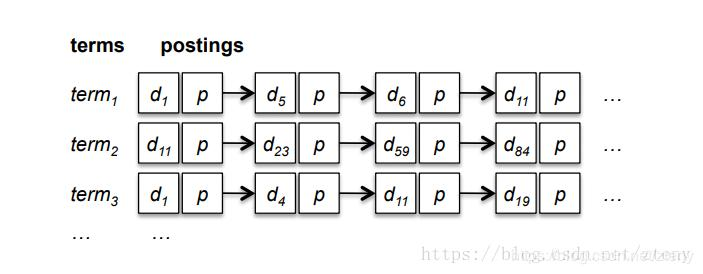
\includegraphics[width=\linewidth]{Images/postings}
%	\captionof{figure}{Positional inverted index}
%\end{Figure}

In this project, the postings for one word are kept in an object of type \verb!Term!. It contains a dictionary, \verb!postings!, where the keys are document IDs where the term appeared and the values are lists of positions in those documents. These lists are kept sorted for the linear merge we perform in the query phase, as described in Section \ref{parsing}. 

\verb!Term! also keeps information about the \textit{document frequency} and \textit{term frequency} of a particular word. This helps in processing free word queries, as described in Section \ref{parsing}.

We count the position of a term \textit{after} we remove the stopwords. This reduces the number of positions in a document considerably and also reduces the time of merging postings.


\subsection{Algorithm} \label{algorithm}
As we read through the collection file, which comes in \verb!xml! form, we keep track of the words and document IDs we have seen so far. A document in the collection contains three tags we are interested in:
\begin{itemize}
	\item \verb!<DOCNO />! - tag containing the document number
	\item \verb!<HEADLINE />! - tag containing the headline of the document
	\item \verb!<TEXT />! - tag containing the acutal body of the document
\end{itemize}
We parse the collection using the \verb!xml.etree! package. From each \verb!HEADLINE! and \verb!TEXT! tag we extract the list of words and we preprocess them as described in Section \ref{preprocessing}. For each word we create a new entry in the \verb!InvertedIndex! dictionary, adding the currently seen document number and all the positions of the document the word appears in. Each time we see a new document for a word, we increase the \textit{document frequency} of the word.

Finally, the user can choose to create a new positional inverted index from a collection and print it to a human-readable file, or load another readily created index from a binary file.

\section{Scoring} \label{scoring}
With simple Boolean or phrase search, the documents retrieved either match or do not match. For a better understanding of the user's needs when they search for a phrase, we use a scoring system to rank the documents that are most likely to satisfy the user's query. 

\subsection{TFIDF}
We consider two metrics to calculate this score. The first one is called \textit{term frequency} and is a count of how many times a term occurs in a document. The more times a term appears in a document, the more important that term is to that document. 

The second measure is \textit{inverse document frequency}. This is derived from a term's \textit{document frequency} - the number of document the term appeared in. The more documents the term is seen in, the lesser its importance in the collection. Alternatively, the higher the \textit{inverse document frequency} of a term, the rarer that term is in the collection. Consequently, the document containing the rare term will have a higher score in the query results.

\textit{TFIDF term weighting} combines the two measures in a single formula:

 \[w_{t,d} = (1 + log_{10}tf(t,d))\cdot log_{10}(\frac{N}{df(t)})\]

Then, for each term in our query, we sum the TFIDF term weights, and we compare this sum for all documents that the terms in the query appear in. 

\[Score(q,d) = \sum_{t\in q\cap d}w_{t,d}\]

The documents displayed to the user are sorted in a descending order by their query score, in the format described in Section \ref{parsing}.

\section{Query parsing} \label{parsing}
There are four types of queries that the system supports, and the user can either enter them manually into the command-line interface or read them from a file. The query terms are preprocessed in the same way that the collection is.

\subsection{Boolean queries}
Boolean queries are of the form:

\[Query \; \rightarrow \; term_1 \; AND \; term_2 \;|\; term_1 \; OR \; term_2\]
\[term \; \rightarrow \; NOT \; term \;|\;word \; | \; phrase \; | \; proximity\]

So we only expect one AND or one OR, but the terms can be negated with NOT and can be either simple words, phrases or proximity searches. 

A simple parsing of the query is performed when the query is read. We first check if the query contains the Boolean keywords. If it does, we split the query by AND and OR and inspect the form of the resulting terms. For terms that represent a phrase of proximity search, we pass them to the \verb!process_phrase_query! function. For terms that start with NOT, we add a \verb!negated! flag and pass the non-negated term to the appropriate processing function.

Finally, if one of the terms of the query is a simple word, we process it in the \verb!process_word_query! function, but if the term contains more than two words, we assume it is a free-word query.

After performing the phrase, proximity or word search for each term, we obtain two lists of relevant documents. If the boolean term of the query is AND, we intersect the two lists, and if the term is OR, we perform a union of the list of documents (handled in Python by set operations). 

If a term is negated, we return all documents apart from the relevant ones for the non-negated term. For this, we keep a local variable \verb!all_documents! in the \verb!InvertedIndex! class, which is just a list of all the document IDs.

\subsection{Phrase and proximity search}
Phrase queries are of the following form, starting with quotation marks:
\["term_1 \; term_2"\]

Proximity queries start with a hashtag and are enclosed in brackets:
\[\#prox\_number(term_1, term_2)\]

We process them in the same function because a phrase search can be written as a proximity search:
\[\#1(term_1, term_2)\]

The linear merge algrithm explained in the lectures is implemented in this function. We retrieve the postings for the two terms and perform a linear search throught the list of documents until we find matching document IDs. We then search through the lists of positions in which the terms appeared in the matching document. At each step we compute the distance between those positions.

If we are performing phrase search, we are looking for a distance of 1. If we are performing a proximity search, we are looking for a distance of \textit{prox\_number}. If we find such matching positions, we append the document ID to the list of relevant documents.

This is one aspect of searching that is heavily influenced by stopword removal. If the index still contains stopwords, documents containing phrases such as \textit{"income and tax"} would not be retrieved if the user is searching for \textit{"income tax"}.

\subsection{Ranked IR}

For free-text queries, we fetch the postings for each of the terms. Then, for each document in each posting, we calculate the scoring function, explained in Section \ref{scoring}. We keep a dictionary of documents and their score for the query, and return a list of sorted documents to the user. The relevant documents are sorted in decreasing order of their score. This way, the user can access the most relevant documents first.

\section{Running a search} \label{search}
This tool is operated from the command line by running:

\begin{lstlisting}[language=bash]
$ python RunSearch.py
\end{lstlisting}

The program will guide the user through the searching process and offer them the option of creating a new index or loading an existing one. They can then enter queries manually or read them from a file.

The collection file needs to be written in TREC style, and the query file needs to contain only one query per line, with the query number as the first one or two characters in the line.

A more detailed description of how to use the system and which packages need to be available on the machine can be found in the README file in the code folder.

\section{Lessons learned}
Implementing this system from scratch gave me and in depth understanding of the algorithms presented in class. Choosing a good data structure for the inverted index was challenging, but OOP concepts helped organise the code better. The code went through two phases of refactoring, to become more usable for next projects.

\section{Improvements} \label{improvements}
There are several improvements that can be brought to the system. 

\subsection{Index storage}
The index could be stored more efficiently using Delta Encoding or B-Trees, the pros and cons of which we discussed in class. Depending on the type of collection we build the index on, we might have different needs for item access or finding small variations of a term. This would also allow us to scale the current system to much bigger indices.

\subsection{Tokenising}
The rules for tokenising can also be changed depending on the collection. One strategy would be to keep the hyphens and the apostrophes for better term matching, and also keep special strings such as @ mentions, hashtags, email addresses and URLs in their original form. For the collection provided for the lab exercises, I noticed it might have been useful to keep numbers intact, such as \textit{10.5bn}, since they are quite a common occurrence.

\subsection{Query parsing}
The current parsing of the queries is quite rigid. An improvement that could also allow more complex boolean queries would be to create a context-free grammar for the queries and build a parser for that. This would give more freedom to the user when formulating queries.

\end{multicols}

\end{document}
